\documentclass[11pt,class=report,crop=false]{standalone}
\usepackage{exo7sv}

\begin{document}

%%%%%%%%%%%%%%%%%%%%%%%%%%%%%%%%%%%%%%%%%%%%%%%%%%%%%%%%%%%%%%%%%%%%%%
%%%%%%%%%%%%%%%%%%%%%%%%%%%%%%%%%%%%%%%%%%%%%%%%%%%%%%%%%%%%%%%%%%%%%%

\entete{Université de Lille}{Mathématiques pour la SVT}

\titre{Fiche 1. \quad Fonctions usuelles} 

\encadre{
\emph{Savoir.}
\begin{itemize}[label=$\square$]
  \item Connaître les fonctions usuelles, leur domaine de définition, leurs limites, l'allure du graphe et leur dérivée.
  \item Maîtriser la fonction exponentielle et la fonction logarithmique.
  \item Réviser ses formules trigonométriques.
\end{itemize}
\emph{Savoir-faire.}
\begin{itemize}[label=$\square$]
  \item Déterminer le domaine de définition d'une fonction.
  \item Savoir utiliser l'égalité $x^\alpha = e^{\alpha\ln(x)}$ dans les deux sens.
\end{itemize}
}



%%%%%%%%%%%%%%%%%%%%%%%%%%%%%%%%%%%%%%%%%%%%%%%%%%%
\subsection*{Domaine de définition}

\begin{itemize}
  \item Une fonction $f$ associe à un réel $x$ un réel noté $f(x)$.
  \item Exemple :
  $$\begin{array}{cccc}
     f : & \Rr & \longrightarrow & \Rr \\
         & x   & \longmapsto & x^2 \\
  \end{array}$$
  Alors $f(3) = 9$, $f(-4)= 16$.
  \item Exemple :
  $$\begin{array}{cccc}
     f : & [0,+\infty[ & \longrightarrow & \Rr      \\
         & x           & \longmapsto     & \sqrt{x} \\
  \end{array}$$
  La fonction n'est pas définie pour des $x<0$.
  \item Le \textbf{domaine de définition} d'une fonction $f$ est l'ensemble des $x$, où l'expression $f(x)$ est définie.

  \emph{Note.} Si on vous donne l'expression d'une fonction $f$,  sans préciser l'ensemble de départ c'est à vous de déterminer le domaine de définition !
  
  \item Exemples : trouvons le domaine de définition des fonctions suivantes.
  $$f(x) = \frac{x-1}{x+1} \qquad \mathcal{D}_f = \Rr \setminus \{-1\} = ]-\infty,-1[ \ \cup \ ]-1,+\infty[$$
  $$f(x) = \frac{1}{x^2-4} \qquad \mathcal{D}_f = \Rr \setminus \{-2,+2\}$$
  $$f(x) = \sqrt{x^2-4} \qquad \mathcal{D}_f = ]-\infty,-2] \ \cup \ [+2,+\infty[$$
\end{itemize}

\subsection*{Fonction polynôme}
\begin{itemize}
  \item Une \textbf{fonction monôme} est définie par $f(x) = x^k$ où $k \in \Nn$ est un entier. 
  \item Le domaine de définition est $\mathcal{D}_f = \Rr$.
  \item La dérivée est \myboxinline{$(x^k)' = kx^{k-1}$}.
  \item Les limites en $+\infty$ et $-\infty$ sont :
  $$\lim_{x\to+\infty} x^k = +\infty
  \qquad \text{ et } \qquad
  \lim_{x\to-\infty} x^k =
  \left\{\begin{array}{ll}
  +\infty & \text{ si $k$ est pair} \\
  -\infty & \text{ si $k$ est impair} \\
  \end{array}\right.$$
  \item Une \textbf{fonction polynôme} est une somme de fonctions monômes. Par exemple, les fonctions définies par $f(x)=x$ et $g(x)=x^3-4x+13$ sont des fonctions polynômes.
\end{itemize}

\begin{center}
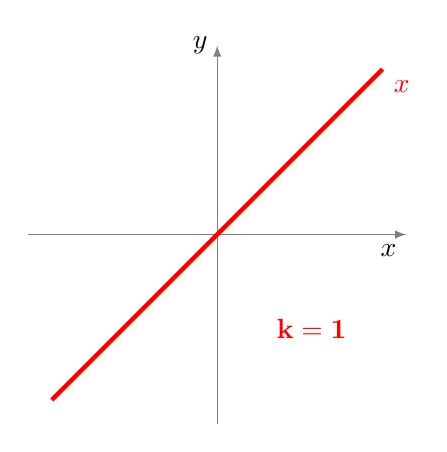
\begin{tikzpicture}[scale=0.6]
      \draw[->,>=latex, gray] (-4,0)--(4,0) node[below left,black] {$x$};
      \draw[->,>=latex, gray] (0,-4)--(0,4) node[left,black] {$y$};
      \draw[ultra thick, color=red,domain=-3.5:3.5,smooth] plot (\x,{\x)}) node[below right]{$x$};
      \node[red] at (2,-2) {$\mathbf{k=1}$};
\end{tikzpicture}\qquad
\begin{tikzpicture}[scale=0.6]
      \draw[->,>=latex, gray] (-4,0)--(4,0) node[below left,black] {$x$};
      \draw[->,>=latex, gray] (0,-4)--(0,4) node[left,black] {$y$};
      \draw[ultra thick, color=red,domain=-1.9:1.9,smooth] plot (\x,{\x*\x)})node[below right]{$x^2$};
      \node[red] at (2,-2) {$\mathbf{k=2}$};
\end{tikzpicture}\qquad
\begin{tikzpicture}[scale=0.6]
      \draw[->,>=latex, gray] (-4,0)--(4,0) node[below left,black] {$x$};
      \draw[->,>=latex, gray] (0,-4)--(0,4) node[left,black] {$y$};
      \draw[ultra thick, color=red,domain=-1.5:1.5,smooth] plot (\x,{\x*\x*\x)})node[below right]{$x^3$};
      \node[red] at (2,-2) {$\mathbf{k=3}$};
\end{tikzpicture}
\end{center}

\subsection*{Fonction inverse}
\begin{itemize}
  \item La \textbf{fonction inverse} est définie par $f(x) = \frac{1}{x}$,
notée aussi $f(x) = x^{-1}$.
  \item Le domaine de définition est $\mathcal{D}_f = \Rr \setminus \{0\}$, car il est interdit de diviser par $0$.
  \item La dérivée est \myboxinline{$\left(\dfrac1x\right)' = -\dfrac{1}{x^2}$}.
  \item Les limites de $f$ sont :
  $$\lim_{x\to-\infty} \frac1x = 0  \qquad 
\lim_{x\to0^-} \frac1x = -\infty  \qquad 
\lim_{x\to0^+} \frac1x = +\infty  \qquad 
\lim_{x\to+\infty} \frac1x = 0$$
\end{itemize}

\begin{center}
\begin{tikzpicture}[scale=1]
      \draw[->,>=latex, gray] (-4,0)--(4,0) node[below left,black] {$x$};
      \draw[->,>=latex, gray] (0,-4)--(0,4) node[left,black] {$y$};
      \draw[ultra thick, color=red,domain=-3.5:-0.3,smooth] plot (\x,{1/\x});
      \draw[ultra thick, color=red,domain=0.3:3.5,smooth] plot (\x,{1/\x}) node[above]{$\frac1x$};
\end{tikzpicture}
\end{center}


\subsection*{Fonction exponentielle}
\begin{itemize}
  \item La \textbf{fonction exponentielle} $f(x) = \exp(x)$ se note aussi par $f(x) = e^x$.
  \item Son domaine de définition est $\mathcal{D}_f = \Rr$.
  \item On a $\exp(x)>0$ pour tout $x\in\Rr$.
  \item $\exp(0) = 1$, $\exp(1)=e \simeq 2.718$.
  \item La dérivée est la fonction elle-même : \myboxinline{$\exp'(x) = \exp(x)$}.
  \item Les limites de $f$ sont :
  $$\lim_{x\to-\infty} e^x = 0  \qquad 
\lim_{x\to+\infty} e^x = +\infty$$
  \item Propriétés :
  \begin{center}
  \myboxinline{$\displaystyle e^{a+b} = e^a \cdot e^b$}\qquad
  \myboxinline{$\displaystyle (e^x)^\alpha = e^{\alpha x}$}\qquad
  \myboxinline{$\displaystyle (e^{-x}) = \frac{1}{e^x}$}
  \end{center}
\end{itemize}

\begin{center}
\begin{tikzpicture}[scale=1]
      \draw[->,>=latex, gray] (-4,0)--(4,0) node[below left,black] {$x$};
      \draw[->,>=latex, gray] (0,-1)--(0,8) node[left,black] {$y$};
      \draw[ultra thick, color=red,domain=-5:2,samples=50,smooth] plot (\x,{exp(\x)}) node[below right]{$\exp(x)$};
	  \fill (0,0) circle (2pt) node[below left]{$0$};
      \fill (0,1) circle (2pt) node[above left]{$1$};
      \coordinate (A) at (1,2.718);
      \fill (A) circle (2pt);
      \fill (A -| 0,0) circle (2pt) node[left]{$e$};
      \fill (A |- 0,0) circle (2pt) node[below]{$1$};
      \draw[dashed](A -| 0,0) -- (A) -- (A |- 0,0);
\end{tikzpicture}
\end{center}


\subsection*{Fonction logarithme}
\begin{itemize}
  \item Le \textbf{logarithme népérien} se note $f(x) = \ln(x)$.
  \item Son domaine de définition est $\mathcal{D}_f = ]0,+\infty[$.
  Le logarithme n'est pas défini pour des $x$ négatifs ou nuls.
  \item $\ln(1) = 0$, \  $\ln(e)=1$.
  \item Propriétés :
  \begin{center}
  \myboxinline{$\displaystyle \ln(a \times b) = \ln(a) + \ln(b)$}\qquad
  \myboxinline{$\displaystyle \ln(x^\alpha) = \alpha \ln(x)$}\qquad
  \myboxinline{$\displaystyle \ln\left(\frac{1}{x}\right) = -\ln(x)$}
  \end{center}

  \item Le logarithme est la bijection réciproque de l'exponentielle :
  \mybox{$\ln(\exp(x)) = x \qquad \text{ pour tout } x\in\Rr$}
  \mybox{$\exp(\ln(x)) = x \qquad \text{ pour tout } x>0$}
  \item La dérivée du logarithme est la fonction inverse \myboxinline{$\ln'(x) = \frac1x$}.
  \item Les limites de $f$ sont :
  $$\lim_{x\to0^+} \ln(x) = -\infty  \qquad 
\lim_{x\to+\infty} \ln(x) = +\infty$$
\end{itemize}

\begin{center}
\begin{tikzpicture}[scale=1]
      \draw[->,>=latex, gray] (-1,0)--(7,0) node[below left,black] {$x$};
      \draw[->,>=latex, gray] (0,-4)--(0,4) node[left,black] {$y$};
      \draw[ultra thick, color=red,domain=0.05:6.5,samples=50,smooth] plot (\x,{ln(\x)}) node[above]{$\ln(x)$};
	  \fill (0,0) circle (2pt) node[below left]{$0$};
      \fill (1,0) circle (2pt) node[below]{$1$};
      \fill (0,1) circle (2pt) node[left]{$1$};
      \coordinate (A) at (2.718,1);
      \fill (A) circle (2pt);
      \fill (A -| 0,0) circle (2pt) node[left]{$1$};
      \fill (A |- 0,0) circle (2pt) node[below]{$e$};
      \draw[dashed](A -| 0,0) -- (A) -- (A |- 0,0);

\end{tikzpicture}
\end{center}


\subsection*{Fonctions puissances}
\begin{itemize}
  \item Les \textbf{fonctions puissances} $f(x) = x^\alpha$, avec $\alpha \in \Rr$ fixé, généralisent les fonctions polynômes (où l'exposant était un entier). 

  \item Elles sont définies par :
  \mybox{$\displaystyle x^\alpha = e^{\alpha \ln(x)}$}
  Autrement dit $x^\alpha = \exp(\alpha \ln(x))$.

  \item Le domaine de définition est $\mathcal{D}_f = ]0,+\infty[$.

  \item La dérivée est \myboxinline{$(x^\alpha)' = \alpha x^{\alpha-1}$}.

  \item Exemple (carré) : $\alpha = 2$, on retrouve la fonction carrée $x^\alpha =  
  e^{2 \ln(x)} = (e^{\ln(x)})^2 = x^2$.
  \item Exemple (racine carrée) : $\alpha = \frac12$, alors $x^{\frac12} = \sqrt{x}$, qui vérifie bien sûr $(x^{\frac12})^2 = x$.
  \item Exemple (racine cubique) : $\alpha = \frac13$, alors $x^{\frac13} = \sqrt[3]{x}$, qui vérifie $(x^{\frac13})^3 = x$.
\end{itemize}

\begin{center}
\begin{tikzpicture}[scale=1]
      \draw[->,>=latex, gray] (-1,0)--(7,0) node[below left,black] {$x$};
      \draw[->,>=latex, gray] (0,-1)--(0,4) node[left,black] {$y$};
      \draw[ultra thick, color=red,domain=0:6.5,samples=100,smooth] plot (\x,{sqrt(\x)}) node[above]{$\sqrt{x} = x^{\frac12}$};
	  \fill (0,0) circle (2pt) node[below left]{$0$};
      \fill (1,0) circle (2pt) node[below]{$1$};
      \fill (0,1) circle (2pt) node[left]{$1$};
      \fill (1,1) circle (2pt);
      \draw[dashed](1,0) -- (1,1) -- (0,1);
\end{tikzpicture}
\end{center}

%%%%%%%%%%%%%%%%%%%%%%%%%%%%%%%%%%%%%%%%%%%%%%%%%%%
\subsection*{Sinus, cosinus, tangente}

\begin{itemize}
  \item Les fonctions \textbf{sinus} et \textbf{cosinus} sont définies sur $\Rr$. 

  \item Les dérivée sont \myboxinline{$\sin'(x) = \cos(x)$} et \myboxinline{$\cos'(x) = -\sin(x)$}.
\end{itemize}

\begin{center}
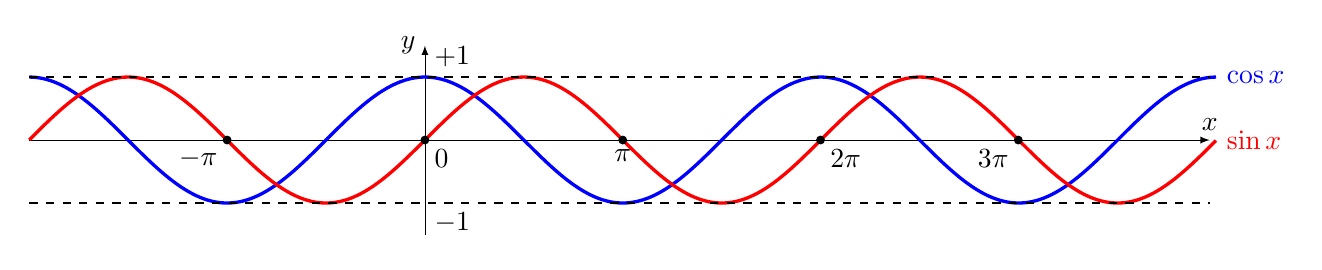
\begin{tikzpicture}[scale=0.8]

	\draw[->,>=latex, black, very thin] (-6.28,0) -- (12.46,0) node[above] {$x$};
	\draw[->,>=latex, black, very thin] (0,-1.5) -- (0,1.5) node[left] {$y$};

	\draw[domain=-6.28:12.56, blue,very thick,samples=200, smooth] plot (\x,{cos(\x r)}) node[right] {$\cos x$};
	\draw[domain=-6.28:12.56, red,very thick, samples=200, smooth] plot (\x,{sin(\x r)}) node[right] {$\sin x$};;

	\draw[dashed] (-6.28,1) -- (12.46,1);
	\draw[dashed] (-6.28,-1) -- (12.46,-1);


	\fill (0,0) circle (2pt) node[below right] {$0$};
	\fill (3.14,0) circle (2pt) node[below] {$\pi$};
	\fill (6.28,0) circle (2pt) node[below right] {$2\pi$};
	\fill (-3.14,0) circle (2pt) node[below left] {$-\pi$};
	\fill (9.42,0) circle (2pt) node[below left] {$3\pi$};

   \node[above right] at (0,1) {$+1$};
   \node[below right] at (0,-1) {$-1$};

\end{tikzpicture}
\end{center}

Voici un zoom sur l'intervalle $[-\pi,\pi]$.
\begin{center}
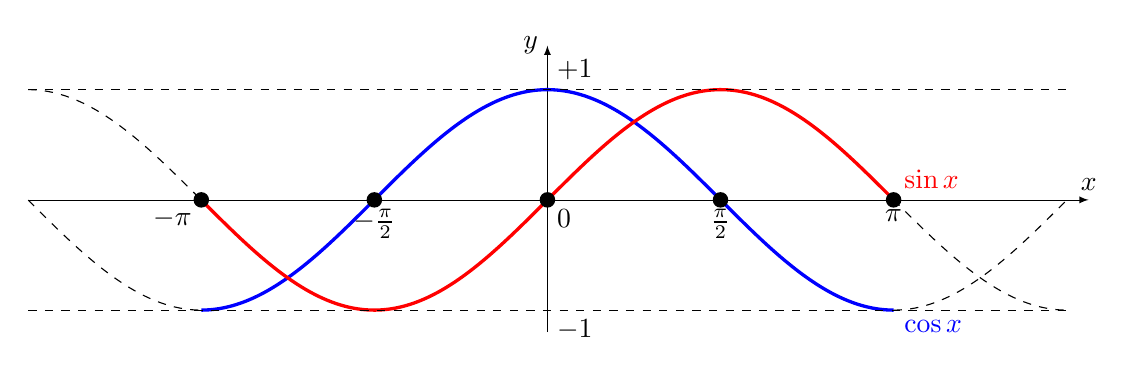
\begin{tikzpicture}[scale=1.4]

	\draw[->,>=latex, black, very thin] (-4.71,0) -- (4.91,0) node[above] {$x$};
	\draw[->,>=latex, black, very thin] (0,-1.2) -- (0,1.4) node[left] {$y$};

	\draw[domain=-3.14:3.14, blue,very thick,samples=200, smooth] plot (\x,{cos(\x r)}) node[below right] {$\cos x$};
	\draw[domain=-3.14:3.14, red,very thick, samples=200, smooth] plot (\x,{sin(\x r)}) node[above right] {$\sin x$};

	\draw[domain=3.14:4.71, black, dashed, samples=50, smooth] plot (\x,{cos(\x r)}) ;
	\draw[domain=3.14:4.71, black, dashed, samples=50, smooth] plot (\x,{sin(\x r)});


	\draw[domain=-4.71:-3.14, black, dashed, samples=50, smooth] plot (\x,{cos(\x r)}) ;
	\draw[domain=-4.71:-3.14, black, dashed, samples=50, smooth] plot (\x,{sin(\x r)});

	\draw[dashed] (-4.71,1) -- (4.71,1);
	\draw[dashed] (-4.71,-1) -- (4.71,-1);

    %\draw[color=blue] plot[id=sin] function{sin(x)}  node[right] {$f(x) = \sin x$};

	\fill (0,0) circle (2pt) node[below right] {$0$};
	\fill (3.14,0) circle (2pt) node[below] {$\pi$};
	\fill (1.57,0) circle (2pt) node[below] {$\frac\pi2$};
	\fill (-3.14,0) circle (2pt) node[below left] {$-\pi$};
	\fill (-1.57,0) circle (2pt) node[below] {$-\frac\pi2$};

   \node[above right] at (0,1) {$+1$};
   \node[below right] at (0,-1) {$-1$};

\end{tikzpicture}
\end{center}

\begin{itemize}
  \item La \textbf{tangente} est définie par \myboxinline{$\tan(x) = \dfrac{\sin(x)}{\cos(x)}$}.
Elle est définie si $\cos(x)\neq0$, c'est-à-dire si $x \neq \frac\pi2 + k\pi$ ($k\in\Zz$). Sa dérivée peut s'écrire de deux façons différentes :
\myboxinline{$\tan'(x) = \frac{1}{\cos^2(x)} = 1+\tan^2(x)$}
\end{itemize}




%%%%%%%%%%%%%%%%%%%%%%%%%%%%%%%%%%%%%%%%%%%%%%%%%%%
\subsection*{Rappels de trigonométrie}

\begin{align*}
& \cos^2 x + \sin^2 x = 1 \\
& \cos(x+2\pi)=\cos x \\
& \sin(x+2\pi)=\sin x \\
\end{align*}

{\small
\renewcommand{\arraystretch}{2.5}
$$
\begin{array}{c|*{5}{c}}
    x     & \qquad 0 \qquad & \qquad \dfrac\pi6 \qquad & \qquad \dfrac\pi 4\qquad
& \qquad \dfrac \pi 3\qquad  &\qquad  \dfrac \pi 2\qquad  \\
\hline
\cos x  \quad & 1 & \dfrac{\sqrt3}{2} & \dfrac{\sqrt2}{2} & \dfrac12 & 0 \\
\hline
\sin x  \quad & 0 &\dfrac12 & \dfrac{\sqrt2}{2} & \dfrac{\sqrt3}{2} & 1\\
\hline
\tan x  \ & 0 & \dfrac{1}{\sqrt{3}} & 1 & \sqrt{3} &
\end{array}
$$
}


\begin{center}
\begin{minipage}{0.45\textwidth}
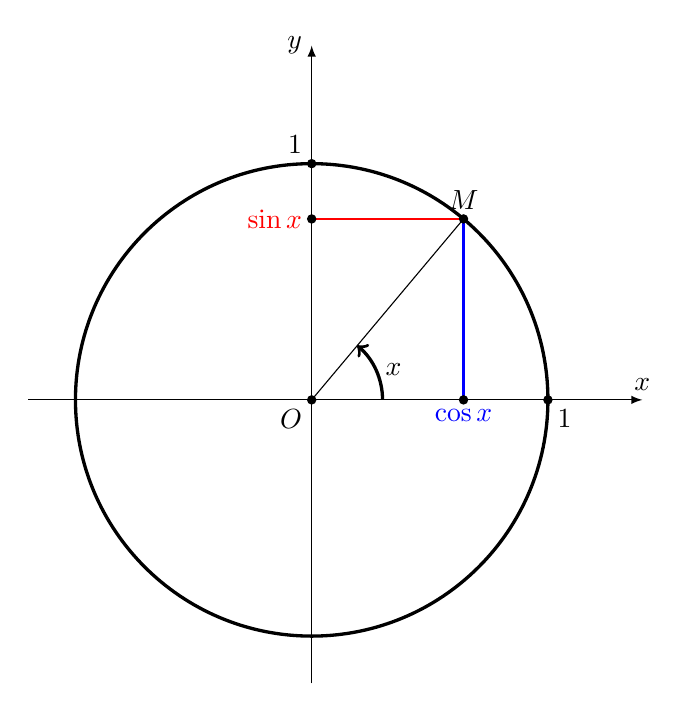
\begin{tikzpicture}[scale=3]

	\draw[->,>=latex, black, thin] (-1.2,0) -- (1.4,0) node[above] {$x$};
	\draw[->,>=latex, black, thin] (0,-1.2) -- (0,1.5) node[left] {$y$};

        % draw the unit circle
        \draw[very thick] (0,0) circle(1);

      \def\x{50};
       \coordinate (M) at ({\x}:1);
       \coordinate (Cos) at ({cos(\x)},0);
       \coordinate (Sin) at (0,{sin(\x)},0);
       \coordinate (Tan) at (1,{sin(\x)/cos(\x)});

       \draw[blue, thick] (M)--(Cos);
       \draw[red, thick] (M)--(Sin);

       	\fill (M) circle (0.02) node[above] {$M$};

        \draw (0,0)--(M);



	\fill (Cos) circle (0.02) node[below, blue] {$\cos x$};
	\fill (Sin) circle (0.02) node[left, red] {$\sin x$};


     \draw[very thick, ->] (0.3,0) arc(0:{\x}:0.3) ;
      \node[right] at ({\x/2}:0.3) {$x$};

	\fill (0,0) circle (0.02) node[below left] {$O$};

     \fill (1,0) circle (0.02) node[below right] {$1$};
     \fill (0,1) circle (0.02) node[above left] {$1$};

%% Tangente
% \beameronly{\uncover<2->}
%{
%    \draw (1,-1.2)--(1,1.5);
%    \draw (0,0)--(Tan)  node[above right] {$T$};
%	\fill (Tan) circle (0.02) ;
%
%
%\begin{scope}[orange, xshift=0.1cm]
%   \draw[<->,>=latex,thick] (1,0)--(1,{sin(\x)/cos(\x)}) node[midway, right] {$\tan x$};
%\end{scope}
%}

\end{tikzpicture}
\end{minipage}\qquad
\begin{minipage}{0.45\textwidth}
\begin{tikzpicture}[scale=4.3,cap=round,>=latex]
 % Unit circle
% Author: Supreme Aryal
% Modified by Arnaud Bodin
% A unit circle with cosine and sine values for some
% common angles.

        % draw the coordinates
       \draw[->] (1cm,0cm) -- (1.2cm,0cm);% node[below] {$x$};
        \draw[->] (0cm,1cm) -- (0cm,1.2cm);% node[left] {$y$};

        % draw the unit circle
        \draw[thick] (1cm,0cm) arc(0:90:1);

        \foreach \x in {30,60} {
                % lines from center to point
                \draw[gray] (0cm,0cm) -- (\x:0.5cm);
                \draw[gray] (\x:0.7cm) -- (\x:0.78cm);
                \draw[gray] (\x:0.92cm) -- (\x:1cm);
                % dots at each point
                \filldraw[black] (\x:1cm) circle(0.4pt);
                % draw each angle in degrees
                \draw (\x:0.6cm) node {$\x^\circ$};
        }
        \foreach \x in {0,45,90} {
                % lines from center to point
                \draw[gray] (0cm,0cm) -- (\x:0.5cm);
                \draw[gray] (\x:0.7cm) -- (\x:0.78cm);
                \draw[gray] (\x:0.92cm) -- (\x:1cm);
                % dots at each point
                \filldraw[black] (\x:1cm) circle(0.4pt);
                % draw each angle in degrees
               \draw (\x:0.6cm) node {$\x^\circ$};
        }
        % draw each angle in radians
        \foreach \x/\xtext in {
            0/0,
            30/\dfrac{\pi}{6},
            45/\dfrac{\pi}{4},
            60/\dfrac{\pi}{3},
            90/\dfrac{\pi}{2}}
                \draw (\x:0.85cm) node {$\xtext$};

        \foreach \x/\xtext/\y in {
            % the coordinates for the first quadrant
            30/\frac{\sqrt{3}}{2}/\frac{1}{2},
            45/\frac{\sqrt{2}}{2}/\frac{\sqrt{2}}{2},
            60/\frac{1}{2}/\frac{\sqrt{3}}{2}}
            % the coordinates for the second quadrant
%             150/-\frac{\sqrt{3}}{2}/\frac{1}{2},
%             135/-\frac{\sqrt{2}}{2}/\frac{\sqrt{2}}{2},
%             120/-\frac{1}{2}/\frac{\sqrt{3}}{2},
%             % the coordinates for the third quadrant
%             210/-\frac{\sqrt{3}}{2}/-\frac{1}{2},
%             225/-\frac{\sqrt{2}}{2}/-\frac{\sqrt{2}}{2},
%             240/-\frac{1}{2}/-\frac{\sqrt{3}}{2},
%             % the coordinates for the fourth quadrant
%             330/\frac{\sqrt{3}}{2}/-\frac{1}{2},
%             315/\frac{\sqrt{2}}{2}/-\frac{\sqrt{2}}{2},
%             300/\frac{1}{2}/-\frac{\sqrt{3}}{2}}
                \draw (\x:1.15cm) node {$\left(\xtext,\y\right)$};

        % draw the horizontal and vertical coordinates
        % the placement is better this way
        \draw %(-1.25cm,0cm) node[above=1pt] {$(-1,0)$}
              (1cm,0cm)  node[above right] {$(1,0)$}
%              (0cm,-1.25cm) node[fill=white] {$(0,-1)$}
              (0cm,1cm)  node[above right] {$(0,1)$};

\end{tikzpicture}
\end{minipage}

\end{center}


\end{document}